% appendices.tex

\chapter{Algorithms and Pseudocode}
\label{app:algorithms}

\renewcommand{\thealgocf}{\thechapter.\arabic{algocf}}
\setcounter{algocf}{0}

This appendix collects compact pseudocode for the attacks and training procedures used in the report. The algorithms use symbolic budgets, step counts, and learning rates; concrete configuration values are defined in Chapter~\ref{chap:experimental_setup}.

\begin{algorithm}[H]
\caption{FGSM-RS}
\DontPrintSemicolon
\KwIn{Model \(f_\theta\), input \(x\), label \(y\), loss \(\ell\), budget \(\varepsilon\), step size \(\alpha\)}
\KwOut{Adversarial input \(x^{\mathrm{adv}}\)}
Sample \(\delta_0 \in \mathcal{S}_\infty(\varepsilon)\)\;
Set \(x_0 \leftarrow \Pi_{[0,1]^d}(x+\delta_0)\)\;
Compute \(g \leftarrow \nabla_x \ell(f_\theta(x_0),y)\)\;
Set \(x^{\mathrm{adv}} \leftarrow \Pi_{(x+\mathcal{S}_\infty(\varepsilon))\cap[0,1]^d}(x_0+\alpha\,\mathrm{sign}(g))\)\;
\Return{\(x^{\mathrm{adv}}\)}
\end{algorithm}

\begin{algorithm}[H]
\caption{PGD Attack}
\DontPrintSemicolon
\KwIn{Model \(f_\theta\), input \(x\), label \(y\), loss \(\ell\), set \(\mathcal{S}_p(\varepsilon)\), step size \(\alpha\), steps \(T\)}
\KwOut{Adversarial input \(x_T^{\mathrm{adv}}\)}
Initialize \(x_0^{\mathrm{adv}}\in (x+\mathcal{S}_p(\varepsilon))\cap[0,1]^d\)\;
\For{\(t=0,\ldots,T-1\)}{
    Compute \(g_t \leftarrow \nabla_x \ell(f_\theta(x_t^{\mathrm{adv}}),y)\)\;
    Take a normalized ascent step using the \(\ell_p\) geometry\;
    Project \(x_{t+1}^{\mathrm{adv}}\) onto \((x+\mathcal{S}_p(\varepsilon))\cap[0,1]^d\)\;
}
\Return{\(x_T^{\mathrm{adv}}\)}
\end{algorithm}

\begin{algorithm}[H]
\caption{CW-\(\ell_2\) Attack}
\DontPrintSemicolon
\KwIn{Model \(f_\theta\), input \(x\), label \(y\), margin loss \(g\), trade-off \(c\), optimizer steps \(T\)}
\KwOut{Adversarial input \(x^{\mathrm{adv}}\)}
Initialize perturbation variable \(\delta\)\;
\For{\(t=1,\ldots,T\)}{
    Minimize \(\|\delta\|_2^2+c\,g(x+\delta)\) by gradient-based optimization\;
    Clip or transform \(x+\delta\) so the candidate remains in \([0,1]^d\)\;
    Keep the best successful adversarial candidate found so far\;
}
\Return{best successful candidate, or the final candidate if none succeeds}
\end{algorithm}

\begin{algorithm}[H]
\caption{DeepFool-\(\ell_2\) Attack}
\DontPrintSemicolon
\KwIn{Model \(f_\theta\), input \(x\), current class \(y\), steps \(T\)}
\KwOut{Adversarial input \(x^{\mathrm{adv}}\)}
Set \(x_0^{\mathrm{adv}}\leftarrow x\)\;
\For{\(t=0,\ldots,T-1\)}{
    \If{\(\arg\max_c f_\theta(x_t^{\mathrm{adv}})_c \neq y\)}{
        \Return{\(x_t^{\mathrm{adv}}\)}
    }
    Linearize the class scores around \(x_t^{\mathrm{adv}}\)\;
    Estimate the closest class boundary under the local linear model\;
    Move \(x_t^{\mathrm{adv}}\) by the corresponding minimal \(\ell_2\) perturbation\;
}
\Return{\(x_T^{\mathrm{adv}}\)}
\end{algorithm}

\begin{algorithm}[H]
\caption{DDN-\(\ell_2\) Attack}
\DontPrintSemicolon
\KwIn{Model \(f_\theta\), input \(x\), label \(y\), loss \(\ell\), initial radius \(\rho_0\), step size \(\alpha\), steps \(T\)}
\KwOut{Adversarial input \(x^{\mathrm{adv}}\)}
Initialize \(\delta_0\) and radius \(\rho_0\)\;
\For{\(t=0,\ldots,T-1\)}{
    Compute \(g_t \leftarrow \nabla_x \ell(f_\theta(x+\delta_t),y)\)\;
    Update perturbation direction using the normalized gradient\;
    \If{\(x+\delta_t\) is adversarial}{
        Decrease the radius for the next candidate\;
    }
    \Else{
        Increase the radius for the next candidate\;
    }
    Normalize the direction to the updated radius and clip to \([0,1]^d\)\;
}
\Return{best successful candidate found during the search}
\end{algorithm}

\begin{algorithm}[H]
\caption{MI-FGSM}
\DontPrintSemicolon
\KwIn{Model \(f_\theta\), input \(x\), label \(y\), loss \(\ell\), budget \(\varepsilon\), step size \(\alpha\), momentum \(\mu\), steps \(T\)}
\KwOut{Adversarial input \(x_T^{\mathrm{adv}}\)}
Initialize \(x_0^{\mathrm{adv}}\leftarrow x\) and \(g_0\leftarrow 0\)\;
\For{\(t=0,\ldots,T-1\)}{
    Compute \(r_t \leftarrow \nabla_x \ell(f_\theta(x_t^{\mathrm{adv}}),y)\)\;
    Set \(g_{t+1}\leftarrow \mu g_t + r_t/\|r_t\|_1\)\;
    Set \(x_{t+1}^{\mathrm{adv}}\leftarrow \Pi_{(x+\mathcal{S}_\infty(\varepsilon))\cap[0,1]^d}(x_t^{\mathrm{adv}}+\alpha\,\mathrm{sign}(g_{t+1}))\)\;
}
\Return{\(x_T^{\mathrm{adv}}\)}
\end{algorithm}

\begin{algorithm}[H]
\caption{TRADES-style Projected Gradient Descent (TPGD)}
\DontPrintSemicolon
\KwIn{Model \(f_\theta\), input \(x\), budget \(\varepsilon\), step size \(\alpha\), steps \(T\)}
\KwOut{Adversarial input \(x_T^{\mathrm{adv}}\)}
Initialize \(x_0^{\mathrm{adv}}\in (x+\mathcal{S}_\infty(\varepsilon))\cap[0,1]^d\)\;
Compute clean prediction \(p_\theta(\cdot\mid x)\)\;
\For{\(t=0,\ldots,T-1\)}{
    Compute \(L_t \leftarrow \operatorname{KL}(p_\theta(\cdot\mid x)\,\|\,p_\theta(\cdot\mid x_t^{\mathrm{adv}}))\)\;
    Ascend \(\nabla_x L_t\) and project onto \((x+\mathcal{S}_\infty(\varepsilon))\cap[0,1]^d\)\;
}
\Return{\(x_T^{\mathrm{adv}}\)}
\end{algorithm}

\begin{algorithm}[H]
\caption{AutoAttack Evaluation Wrapper}
\DontPrintSemicolon
\KwIn{Model \(f_\theta\), evaluation set \(\mathcal{D}_{\mathrm{test}}\), AutoAttack component suite \(\mathcal{A}_{\mathrm{AA}}\)}
\KwOut{AutoAttack robust accuracy}
Initialize success indicator \(s_i\leftarrow 1\) for each test example\;
\For{each component attack \(A\in\mathcal{A}_{\mathrm{AA}}\)}{
    Generate adversarial candidates \(A(x_i,y_i,f_\theta)\)\;
    Set \(s_i\leftarrow 0\) for examples misclassified by the component attack\;
}
Compute robust accuracy \(\frac{1}{|\mathcal{D}_{\mathrm{test}}|}\sum_i s_i\)\;
\Return{robust accuracy}
\end{algorithm}

\begin{algorithm}[H]
\caption{Multi-AT Training}
\DontPrintSemicolon
\KwIn{Training set \(\mathcal{D}_{\mathrm{train}}\), model \(f_\theta\), source attack set \(\mathcal{E}_{\mathrm{src}}\), loss \(\ell\), learning rate \(\eta_\theta\)}
\KwOut{Trained model \(f_\theta^\ast\)}
\For{each training epoch}{
    \For{each minibatch \(\mathcal{B}\)}{
        Assign examples in \(\mathcal{B}\) uniformly across attacks in \(\mathcal{E}_{\mathrm{src}}\)\;
        Generate adversarial examples using the assigned source attack\;
        Compute the uniform mean adversarial loss over the minibatch\;
        Update \(\theta\) using the model optimizer and learning rate \(\eta_\theta\)\;
    }
}
\Return{\(f_\theta^\ast\)}
\end{algorithm}

\begin{algorithm}[H]
\caption{AttackDRO Training}
\DontPrintSemicolon
\KwIn{Training set \(\mathcal{D}_{\mathrm{train}}\), model \(f_\theta\), source attack set \(\mathcal{E}_{\mathrm{src}}\), attack weights \(q\), learning rates \(\eta_\theta,\eta_q\)}
\KwOut{Trained model \(f_\theta^\ast\)}
Initialize \(q\) uniformly over source attack identities\;
\For{each training epoch}{
    \For{each minibatch}{
        Generate adversarial examples using the source attacks\;
        Estimate loss or difficulty for each source attack group\;
        Compute the attack-weighted Group DRO loss using \(q\)\;
        Update \(\theta\) with the weighted loss\;
        Update \(q\) using exponentiated-gradient reweighting over attack groups\;
    }
}
\Return{\(f_\theta^\ast\)}
\end{algorithm}

\begin{algorithm}[H]
\caption{Cluster-DRO and AttackDRO++ Training Overview}
\DontPrintSemicolon
\KwIn{Training set \(\mathcal{D}_{\mathrm{train}}\), model \(f_\theta\), source attacks \(\mathcal{E}_{\mathrm{src}}\), cluster count \(K\), anchor weight \(\lambda_{\mathrm{DRO}}\), group weights \(q\)}
\KwOut{Trained model \(f_\theta^\ast\)}
Initialize feature bank, clusterer, and uniform group weights \(q\)\;
\For{each training epoch}{
    Refresh latent clusters from the feature bank when the refresh condition is met\;
    \For{each minibatch}{
        Generate source adversarial examples as in Multi-AT\;
        Extract representations and, for AttackDRO++, augmented clustering features with gradient fingerprints\;
        Assign each adversarial example to a latent cluster\;
        Compute the uniform adversarial loss over the minibatch\;
        Compute the Cluster-DRO loss using cluster weights \(q\)\;
        Combine the uniform anchor and Cluster-DRO terms using \(\lambda_{\mathrm{DRO}}\)\;
        Update model parameters and then update \(q\) from cluster-level difficulty estimates\;
        Add detached augmented features to the feature bank\;
    }
}
\Return{\(f_\theta^\ast\)}
\end{algorithm}


%===========================================================
% APPENDIX B: EXPERIMENTAL LOGS AND CONFIGURATIONS
%===========================================================

\chapter{Experimental Logs and Configurations}
\label{app:logs}

\begin{figure}[p]
\centering
\captionsetup{font=footnotesize}
\begin{subfigure}[t]{0.45\linewidth}
\centering
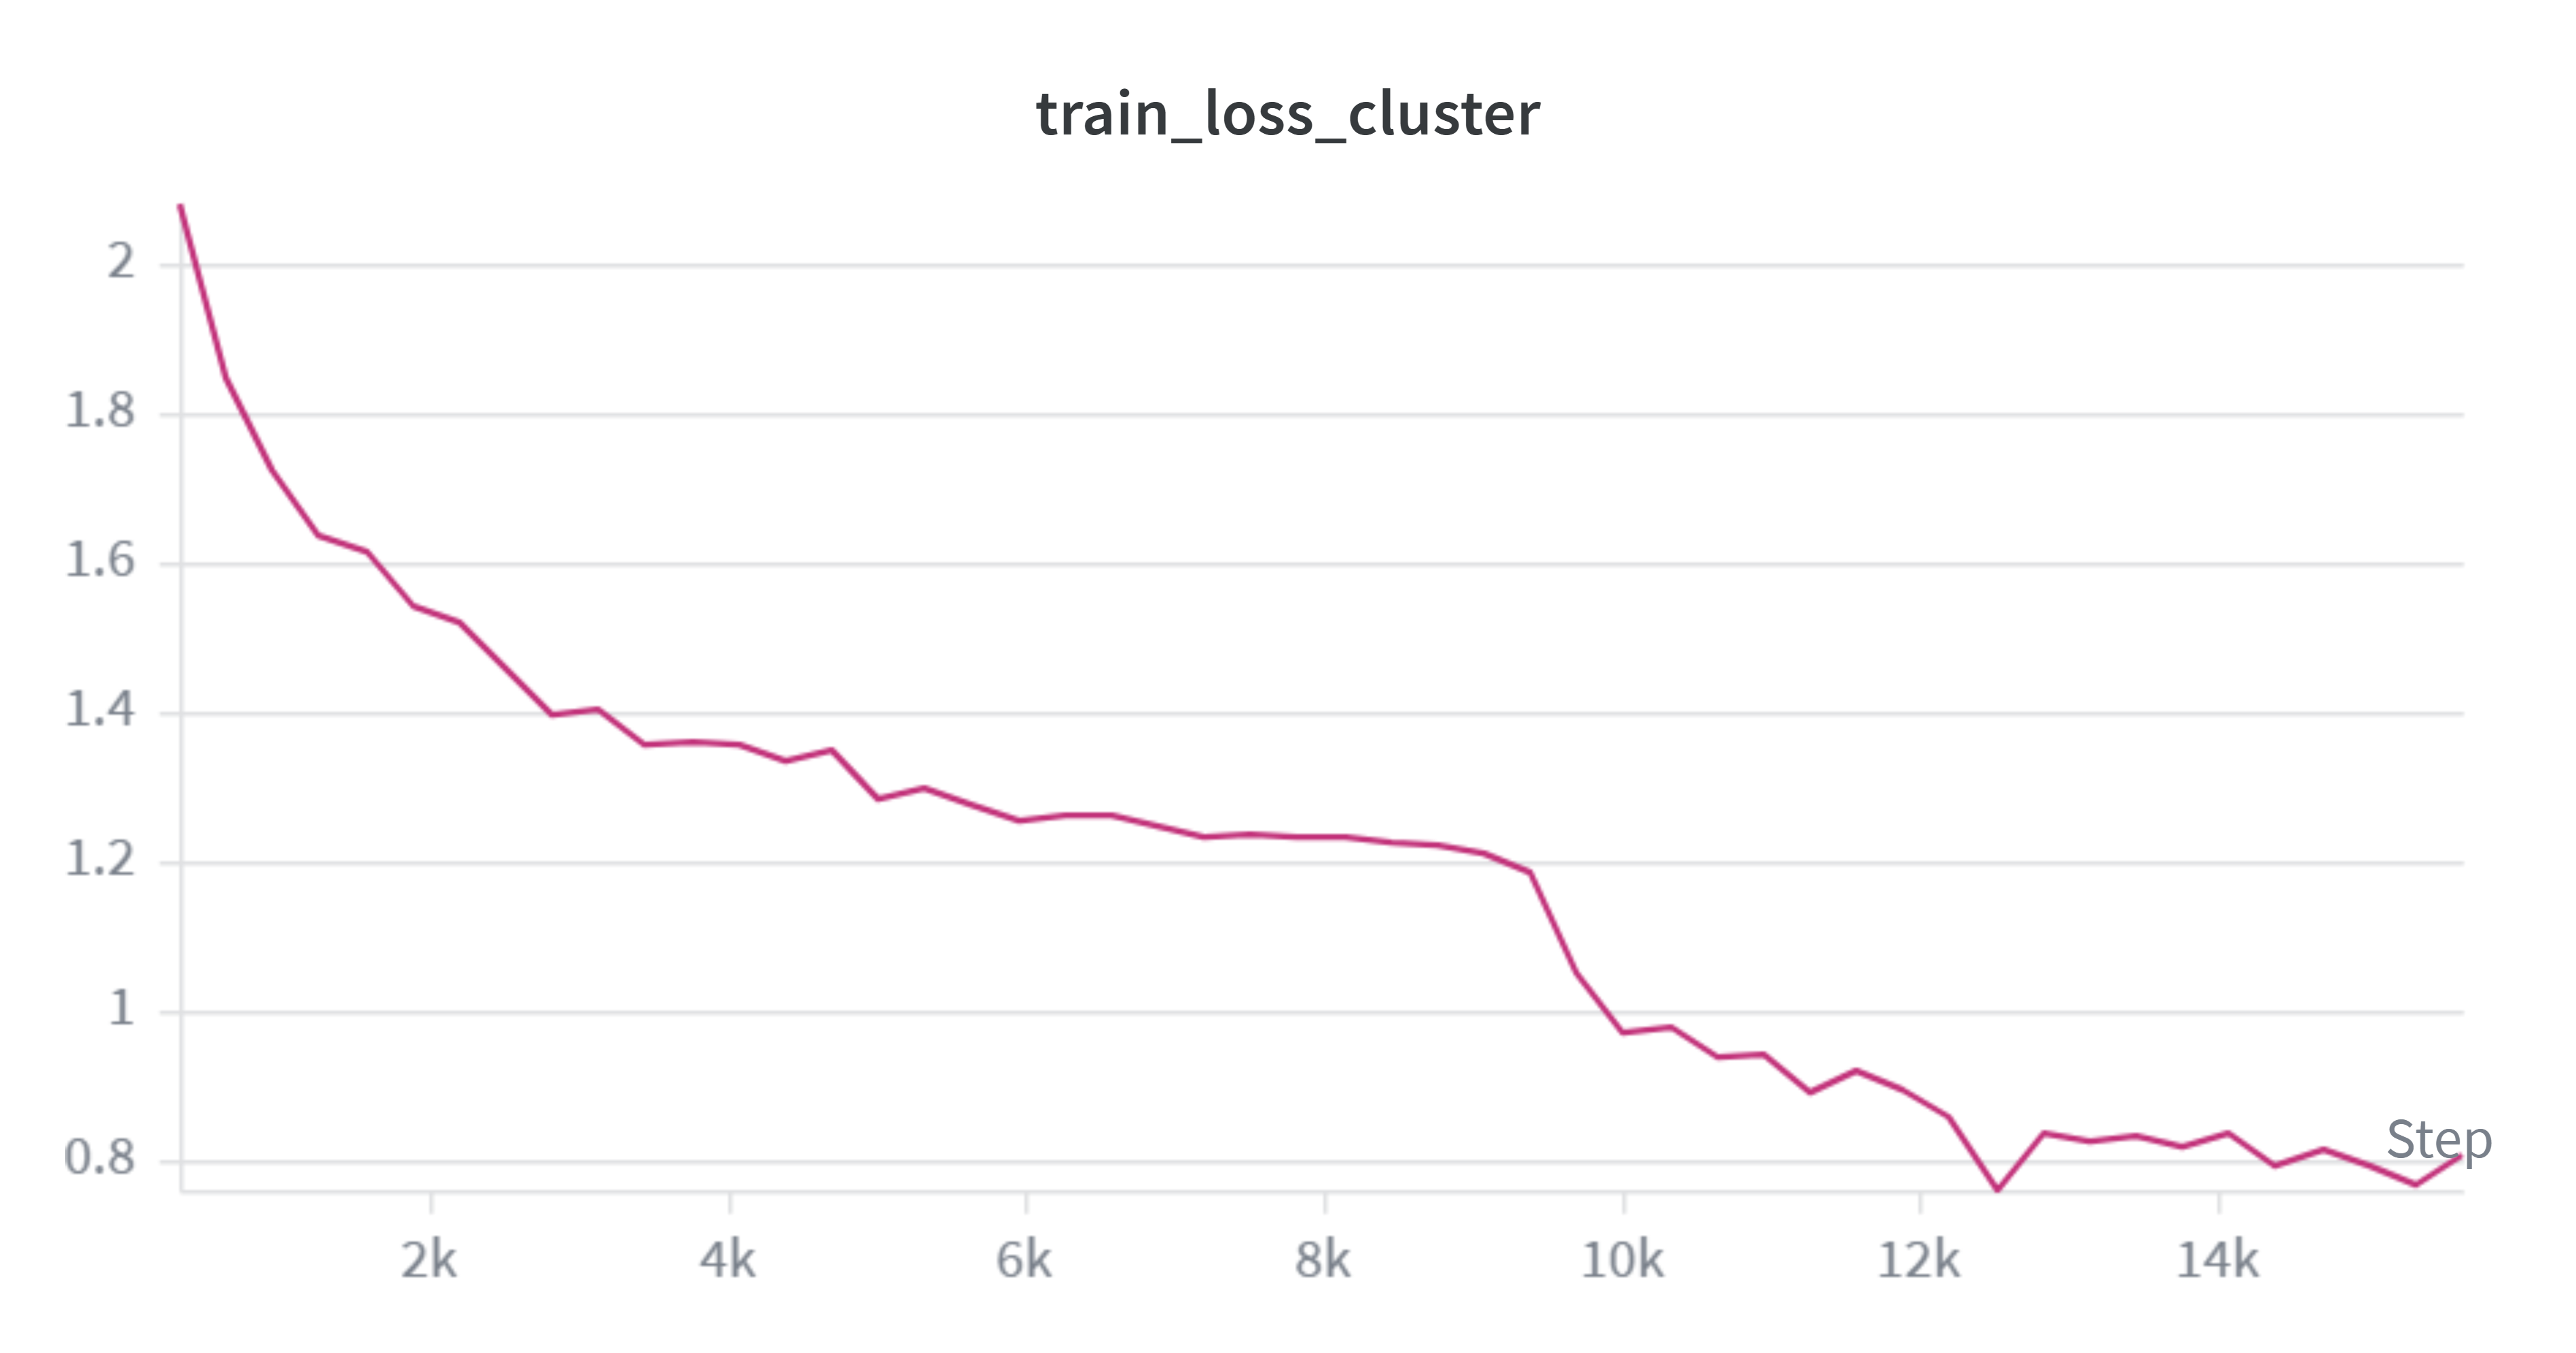
\includegraphics[width=0.95\linewidth]{figures/wandb/wb_train_loss.png}
\caption{Training loss.}
\end{subfigure}
\hfill
\begin{subfigure}[t]{0.45\linewidth}
\centering
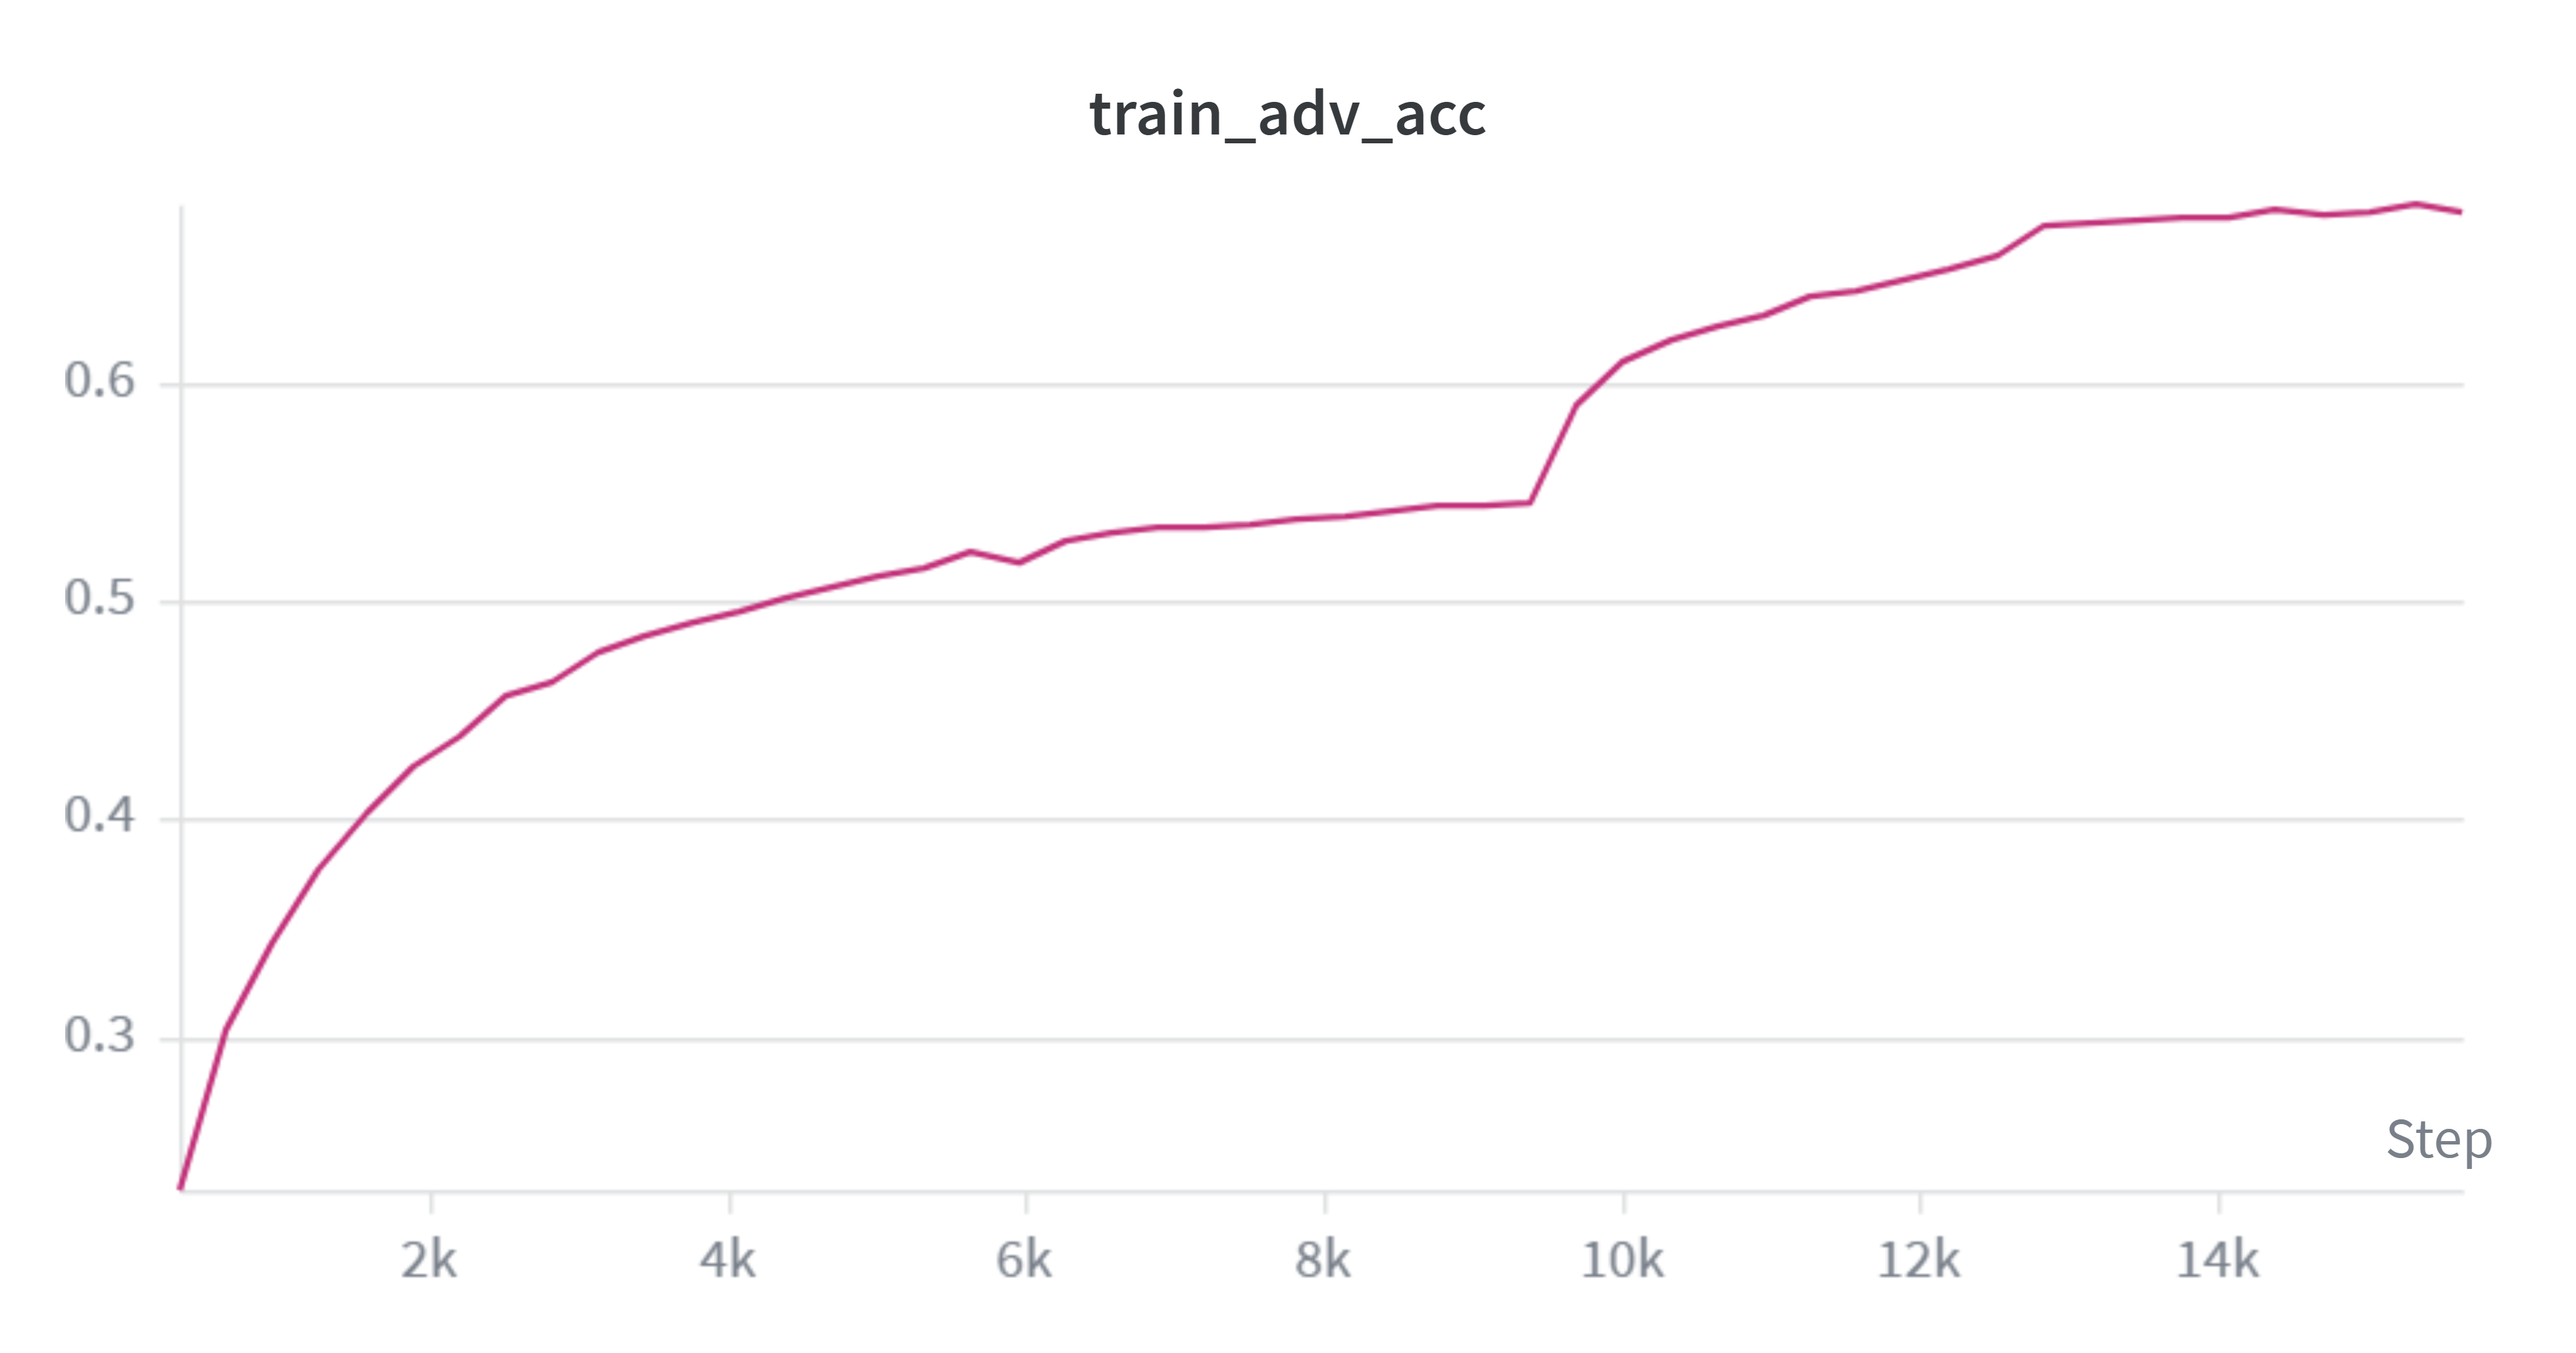
\includegraphics[width=0.95\linewidth]{figures/wandb/wb_train_acc.png}
\caption{Training accuracy.}
\end{subfigure}

\vspace{0.35em}
\begin{subfigure}[t]{0.45\linewidth}
\centering
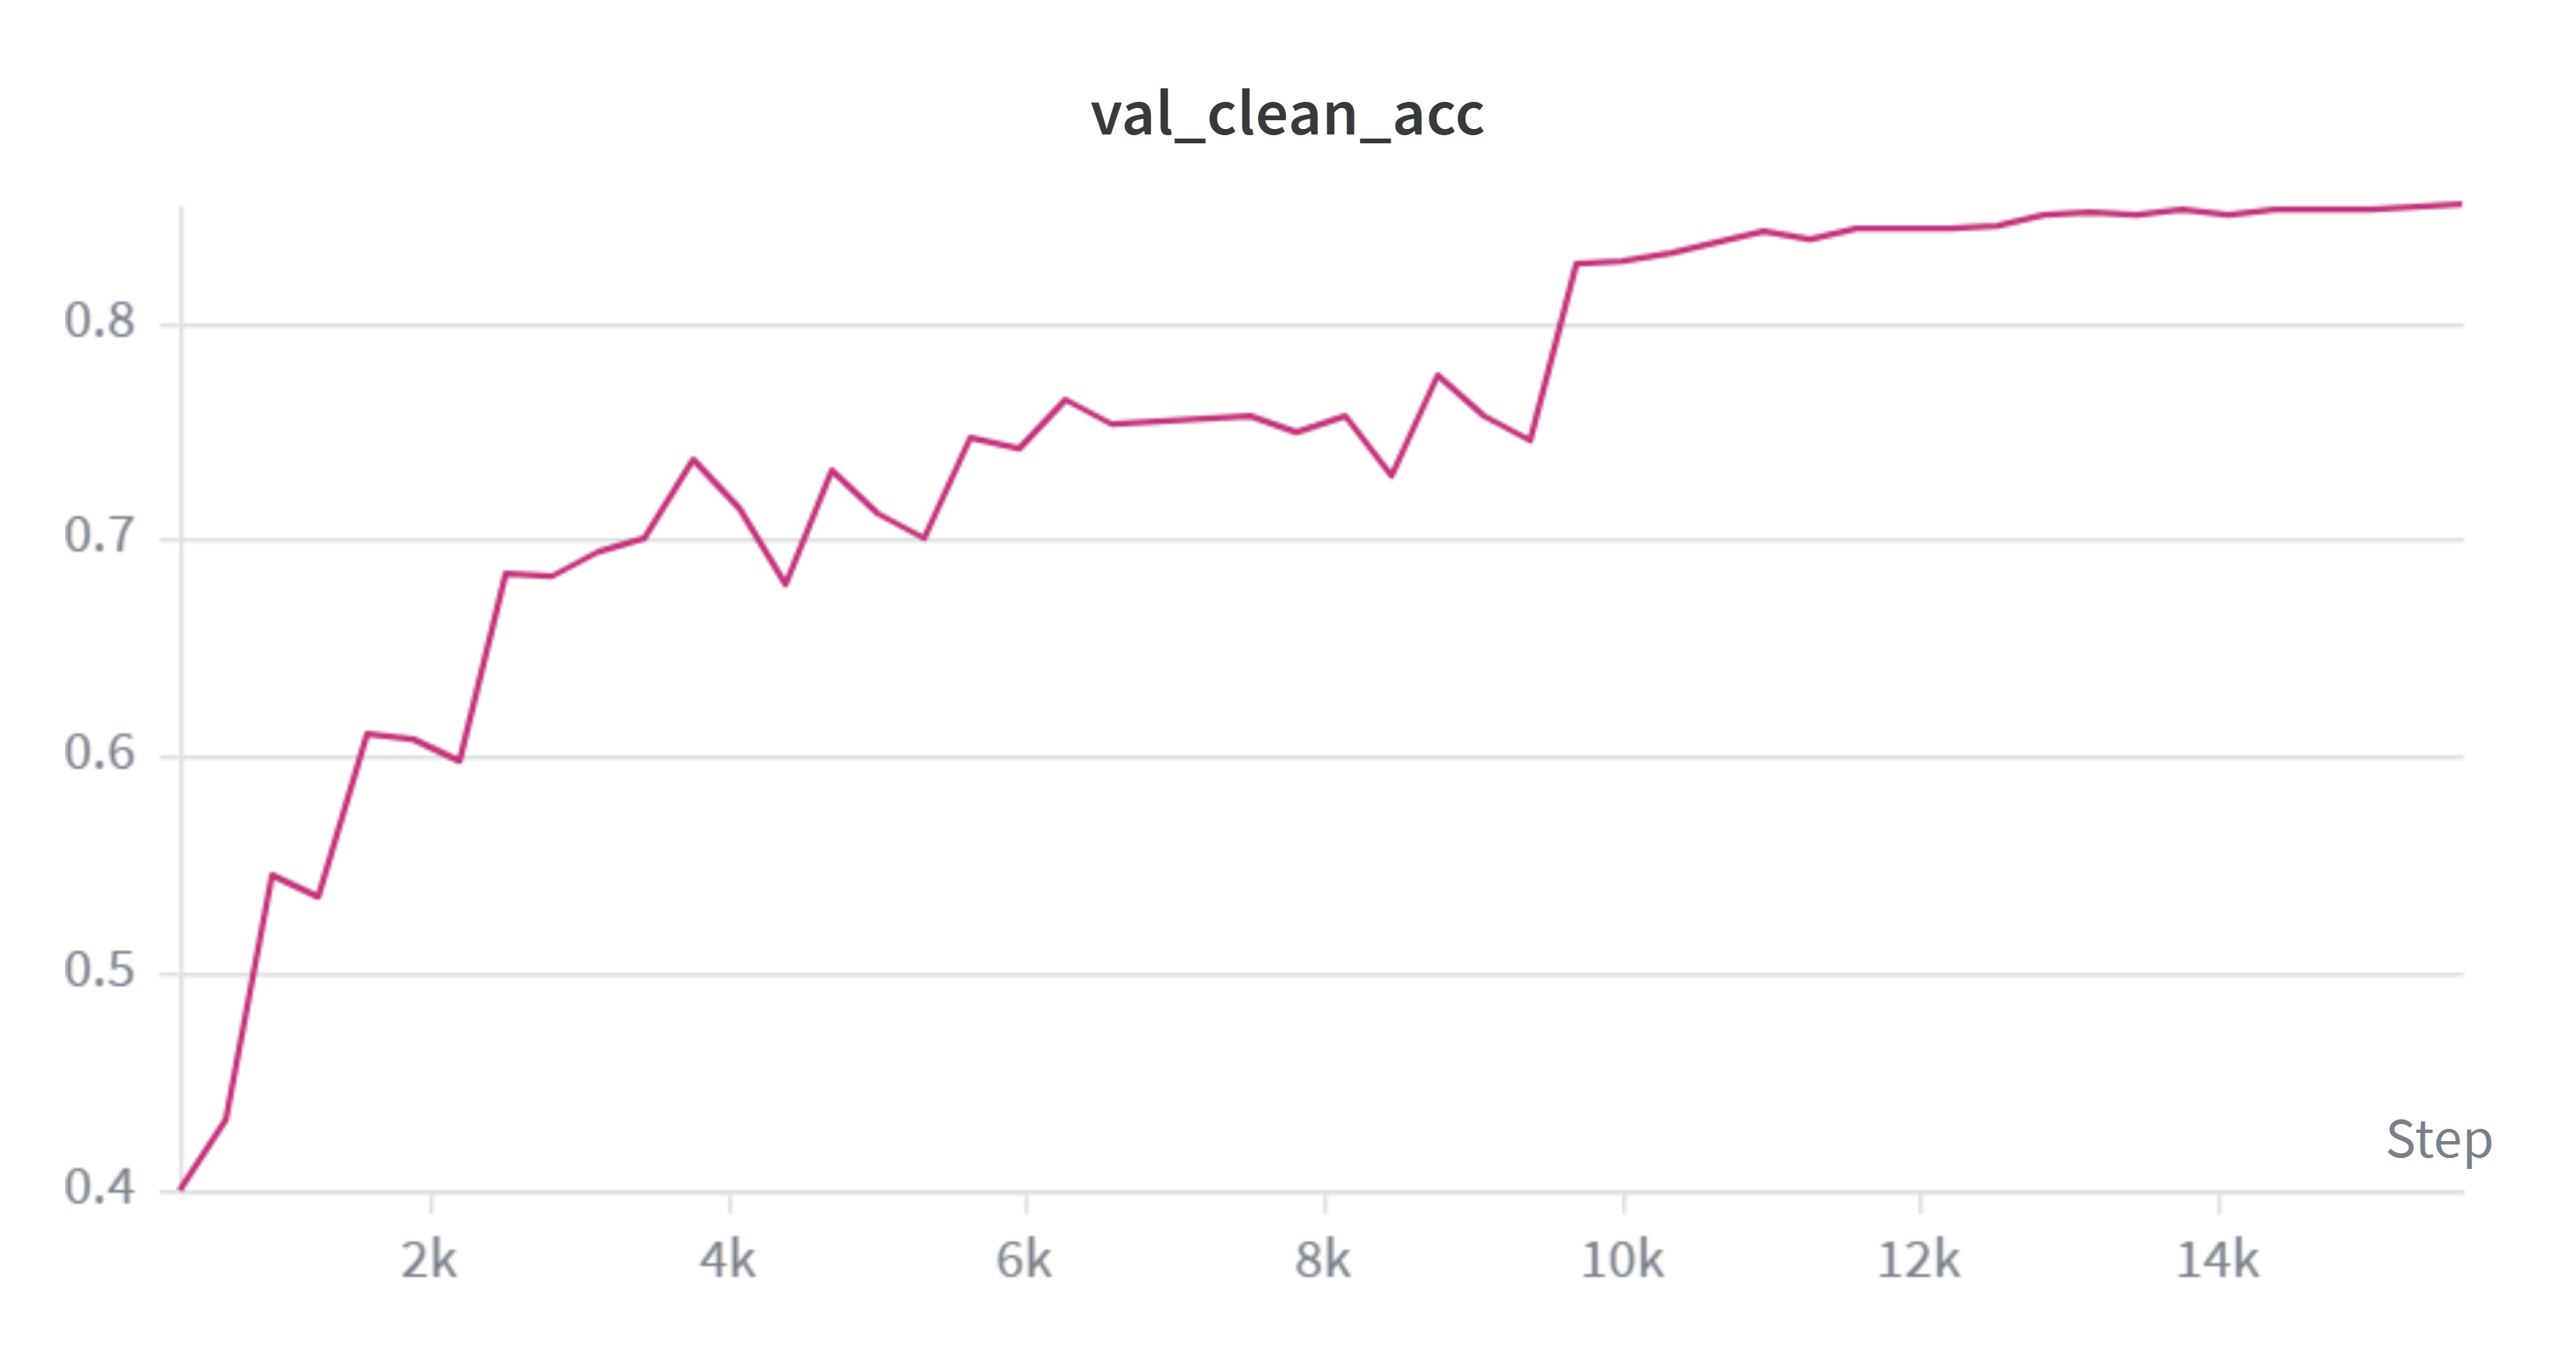
\includegraphics[width=0.95\linewidth]{figures/wandb/wb_val_clean_acc.png}
\caption{Clean validation accuracy.}
\end{subfigure}
\hfill
\begin{subfigure}[t]{0.45\linewidth}
\centering
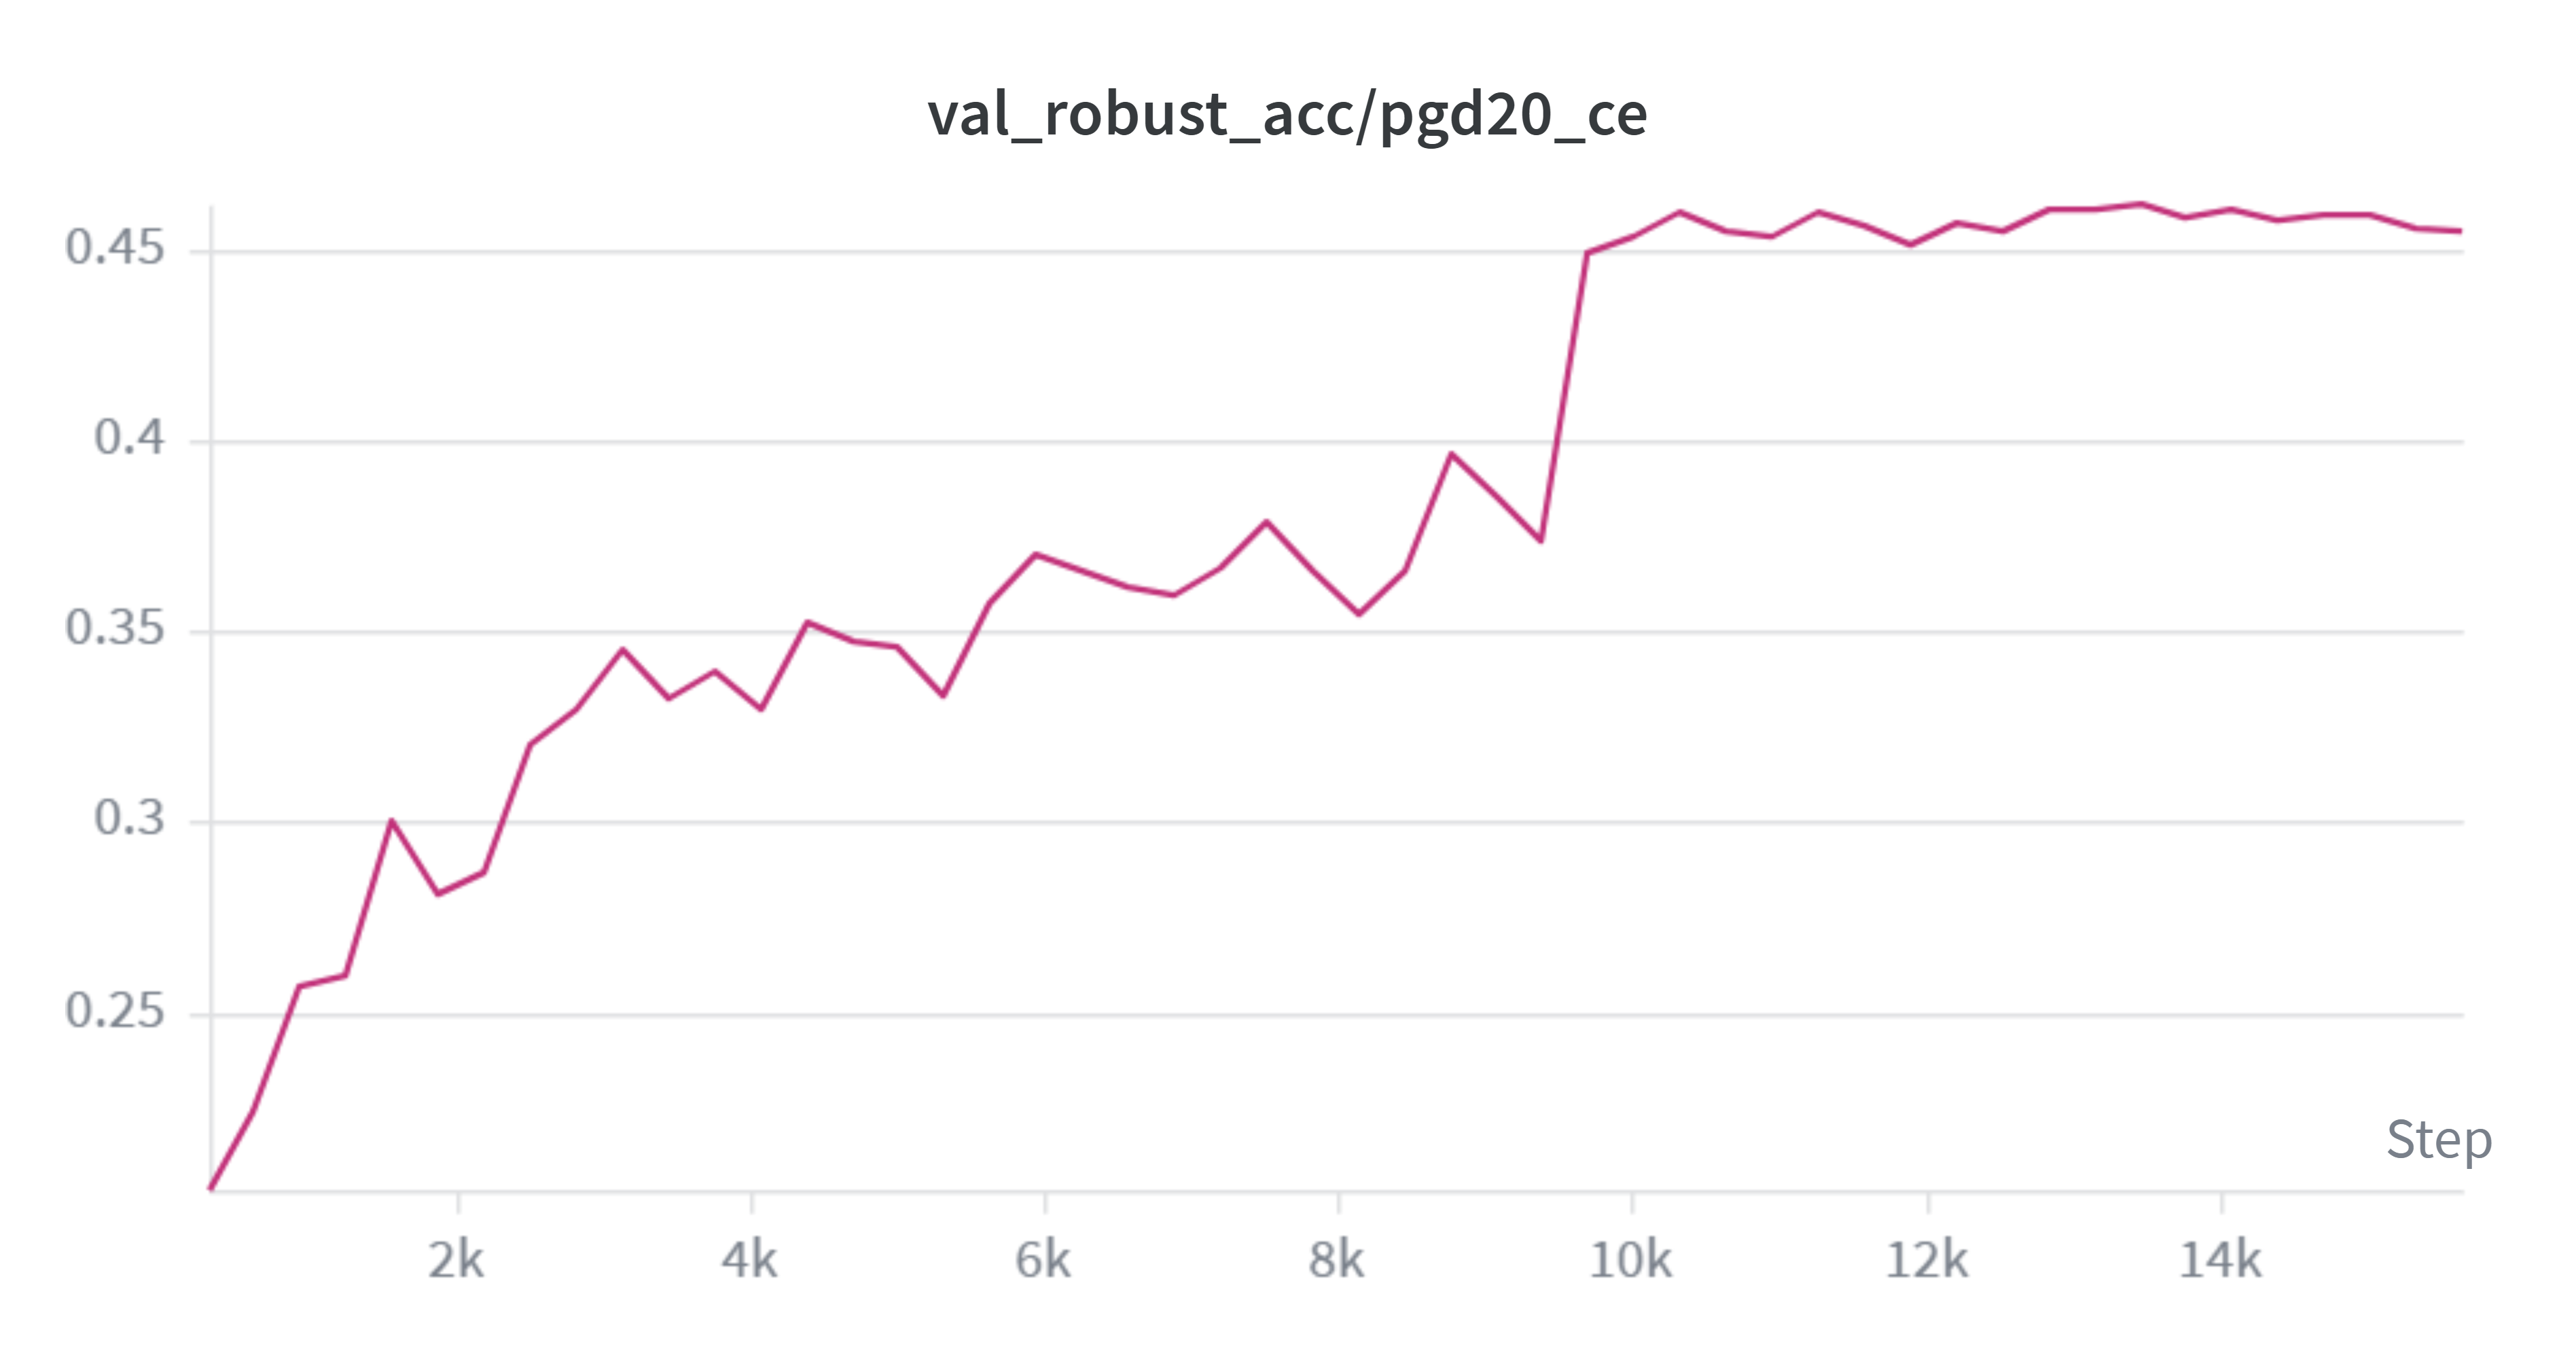
\includegraphics[width=0.95\linewidth]{figures/wandb/wb_pgd_linf_acc.png}
\caption{PGD-$\ell_\infty$ validation accuracy.}
\end{subfigure}

\vspace{0.35em}
\begin{subfigure}[t]{0.45\linewidth}
\centering
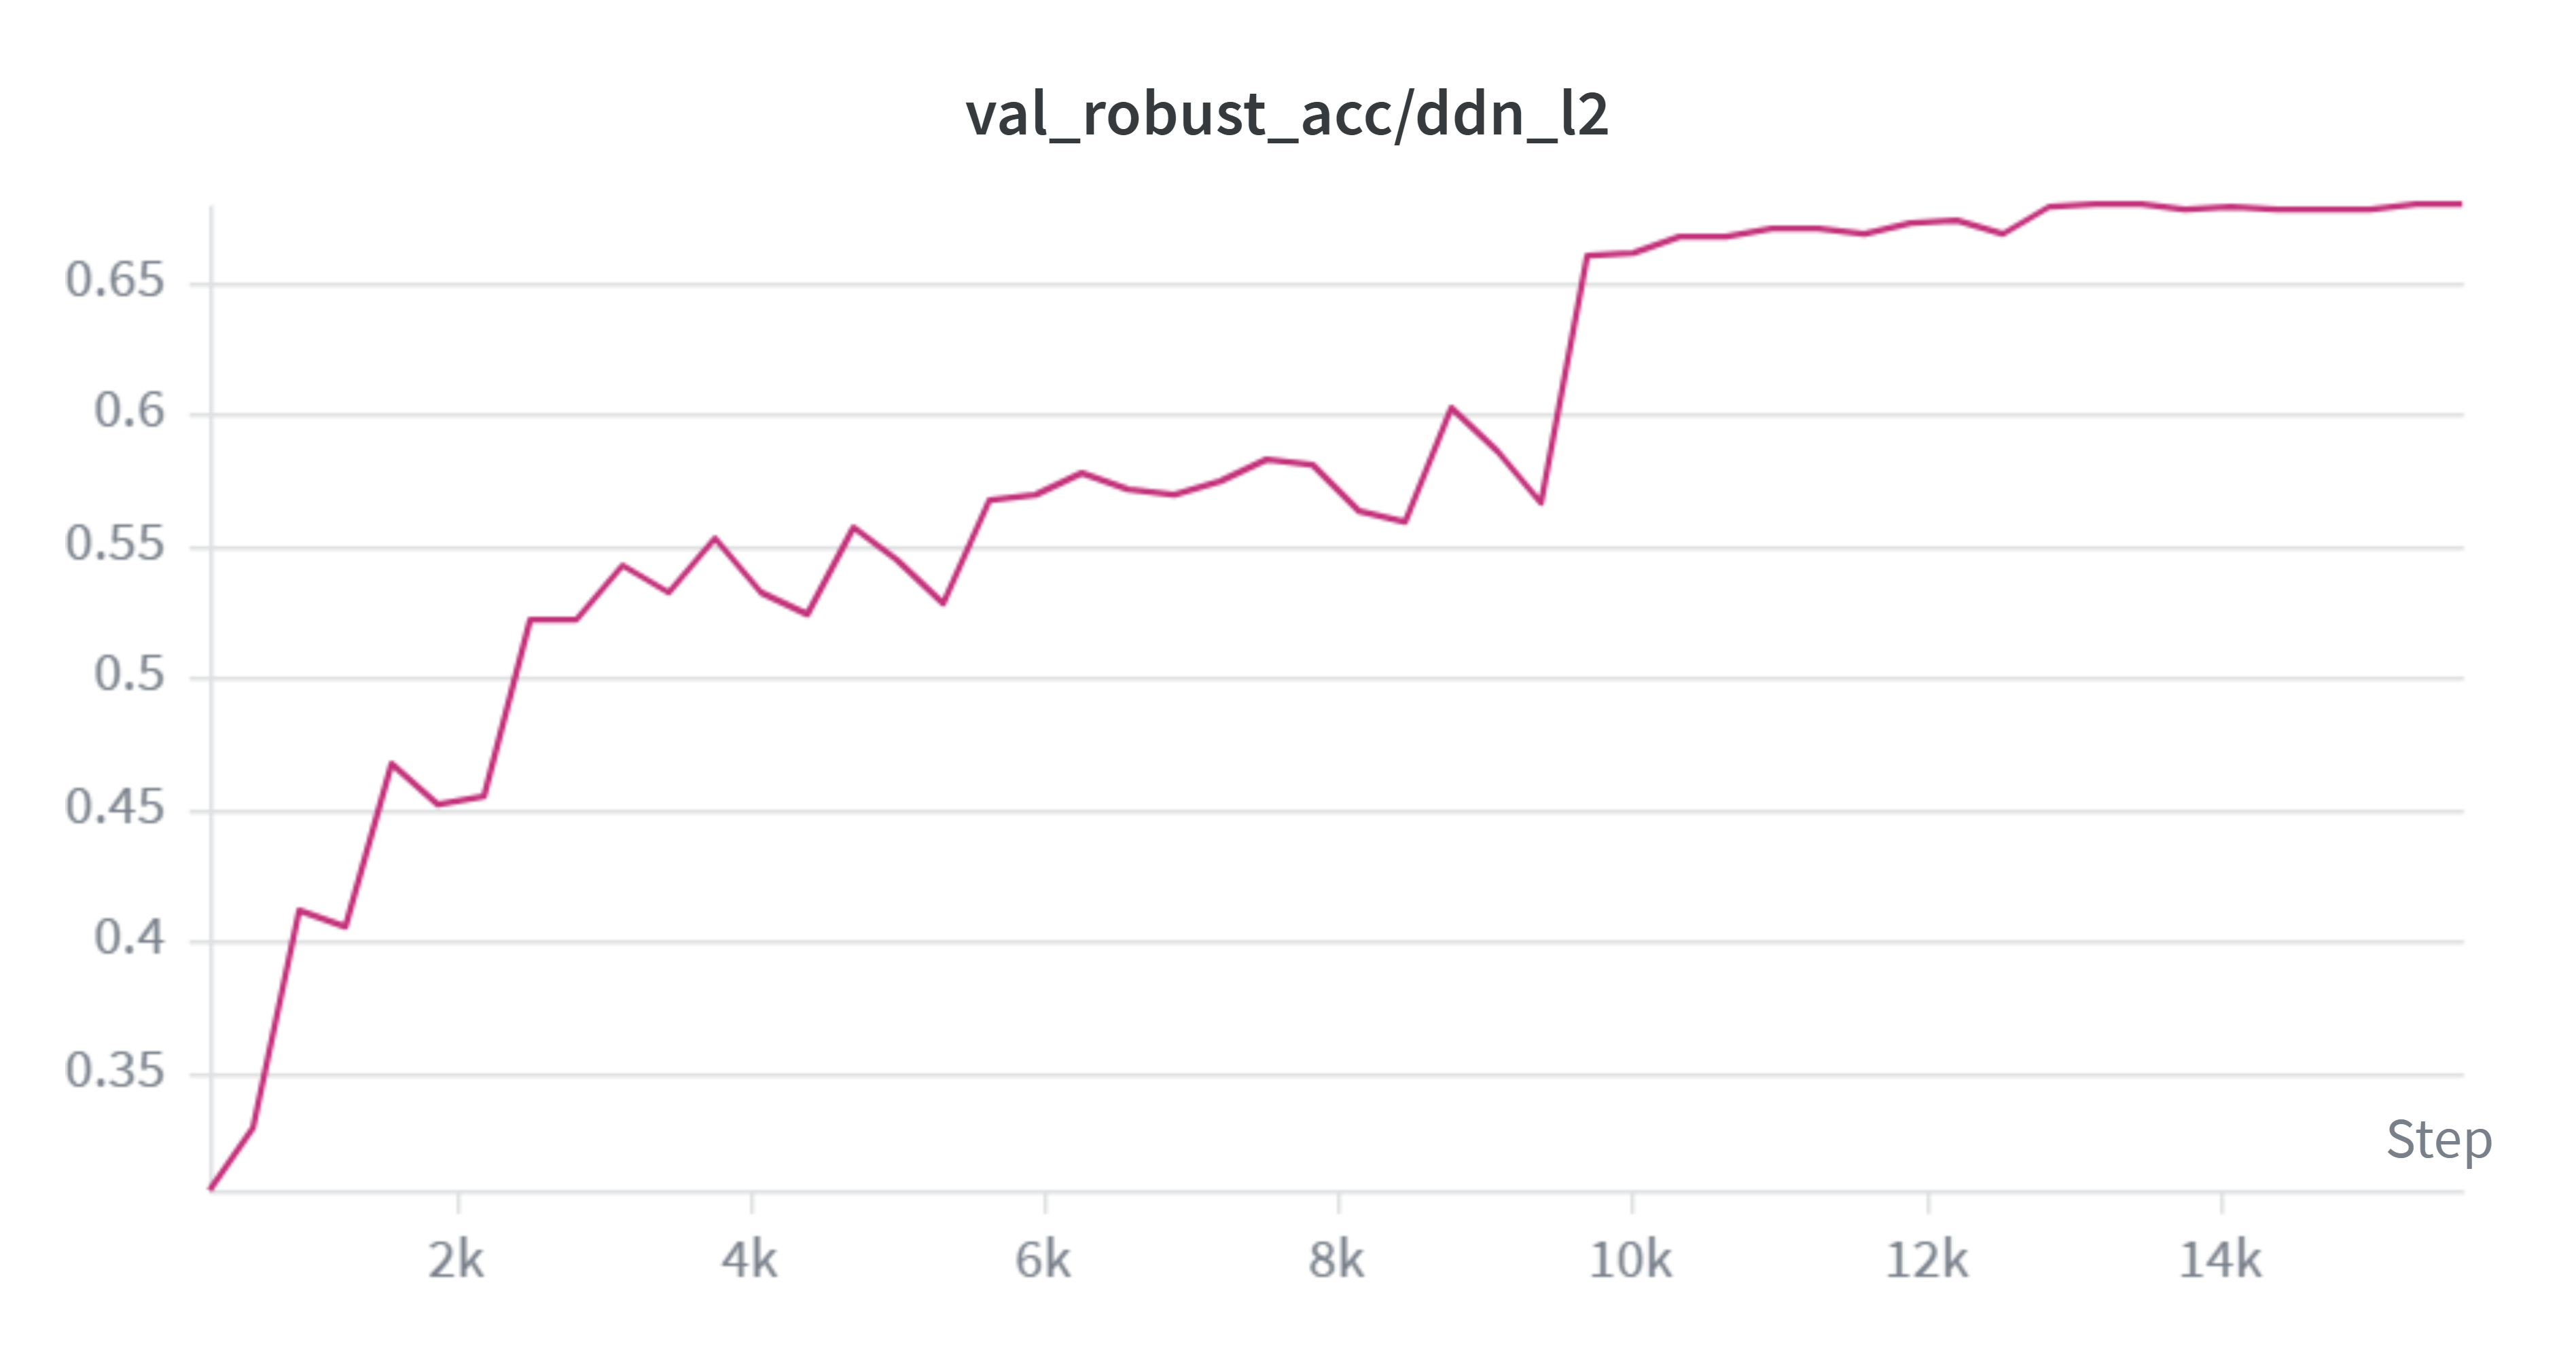
\includegraphics[width=0.95\linewidth]{figures/wandb/wb_ddn_l2_acc.png}
\caption{DDN-$\ell_2$ validation accuracy.}
\end{subfigure}
\hfill
\begin{subfigure}[t]{0.45\linewidth}
\centering
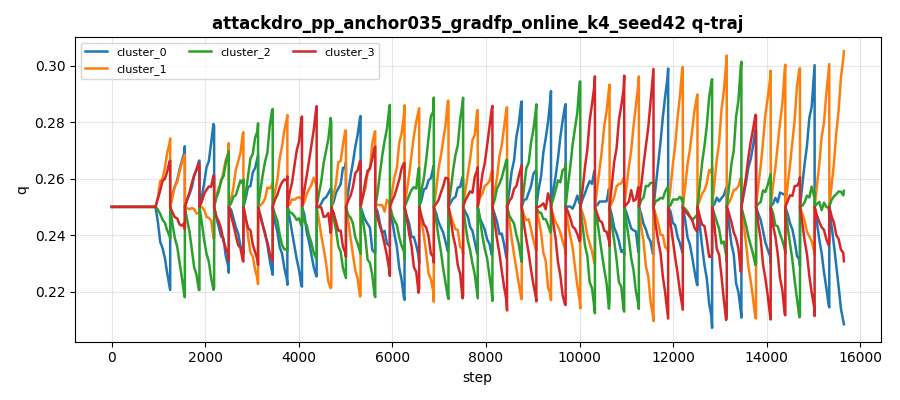
\includegraphics[width=0.95\linewidth]{figures/wandb/media_images_media_q_trajectory_15650_2752bccd0ffdd754ab89.png}
\caption{Group-weight trajectory.}
\end{subfigure}
\caption[W\&B dashboard exports]{Representative W\&B dashboard exports for experiment tracking. Panels (a)\textendash(e) track training loss, training accuracy, clean validation accuracy, and validation robustness under PGD-$\ell_\infty$ and DDN-$\ell_2$ during a training run. Panel (f) records the AttackDRO++ group-weight trajectory diagnostic. These exports document training telemetry and are not used as result evidence.}
\label{fig:app_wandb_core_metrics}
\end{figure}

% Goal: store run configuration, seed policy, split policy, attack configuration,
% training schedule, JSON logs, command lines if available, and compact config tables.

%===========================================================
% APPENDIX C: ADDITIONAL TABLES AND VISUALIZATIONS
%===========================================================

\chapter{Additional Tables and Visualizations}
\label{app:extras}

% Goal: store supplementary ablation tables, sweep summaries, training curves,
% qualitative grids, and plots that are not part of the main chapters.

\section{Adversarial Perturbation Visualizations}
\label{app:adv_visualizations}

\subsection{Grouped Adversarial Perturbation Visualizations}

Figure~\ref{fig:app_grouped_linf_adv_viz} and Figure~\ref{fig:app_grouped_l2_adv_viz} summarize adversarial examples and normalized perturbation heatmaps across the main \(\ell_\infty\) and \(\ell_2\) evaluation attacks. These figures are intended as qualitative support for the attack descriptions in Chapter~2; all heatmaps are normalized for visibility.

\begin{figure}[htbp]
\centering
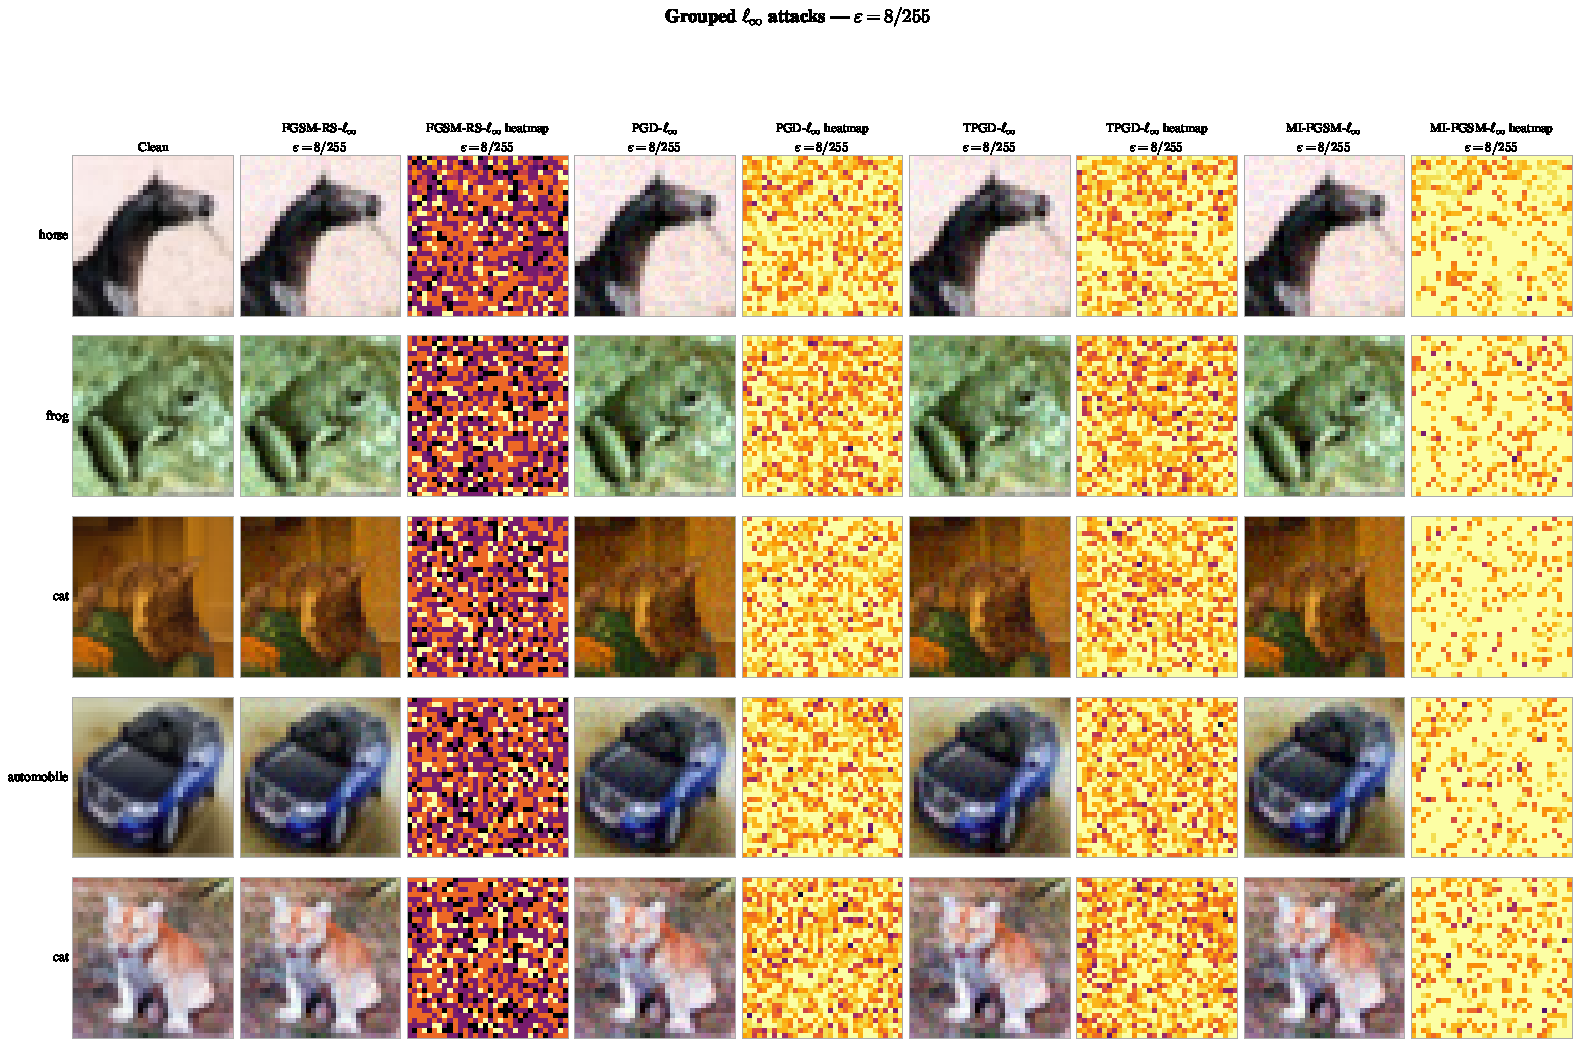
\includegraphics[width=0.90\textwidth]{figures/adv_viz/adv_grouped_linf.pdf}
\caption[Grouped \(\ell_\infty\) perturbation visualization]{Grouped \(\ell_\infty\) adversarial examples on CIFAR-10, with adversarial images and normalized perturbation heatmaps.}
\label{fig:app_grouped_linf_adv_viz}
\end{figure}

\begin{figure}[htbp]
\centering
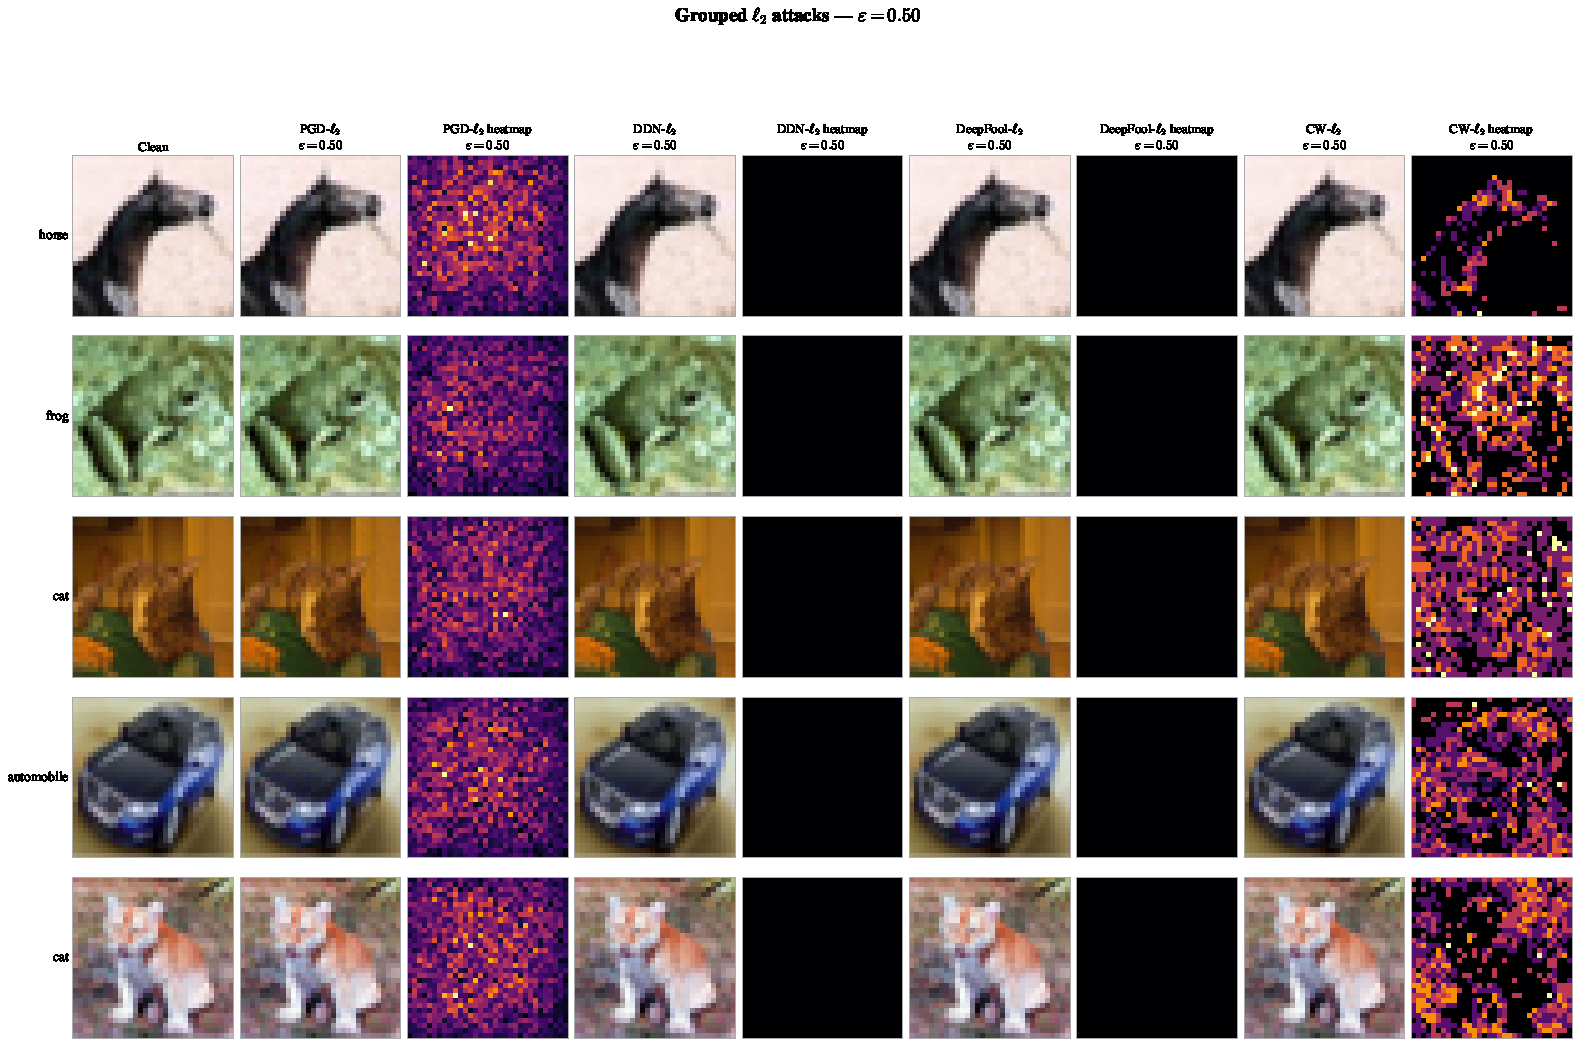
\includegraphics[width=0.90\textwidth]{figures/adv_viz/adv_grouped_l2.pdf}
\caption[Grouped \(\ell_2\) perturbation visualization]{Grouped \(\ell_2\) adversarial examples on CIFAR-10, with adversarial images and normalized perturbation heatmaps.}
\label{fig:app_grouped_l2_adv_viz}
\end{figure}

\begin{table}[H]
\centering
\caption[Supplementary WRN-28-10 architecture check]{Supplementary WRN-28-10 architecture check on CIFAR-10. Values are
robust accuracy (\%) from a single run and are therefore not included in the
main paired claims. Mean(8) and Worst(8) are computed over the eight
non-AutoAttack attacks; AutoAttack-$\ell_\infty$ is reported separately. Bold values indicate the best method for each metric.}
\label{tab:app_wrn2810_architecture_check}
\small
\setlength{\tabcolsep}{4pt}
\renewcommand{\arraystretch}{1.08}
\begin{tabular}{lccc}
\toprule
Method & Mean(8) $\uparrow$ & Worst(8) $\uparrow$ & AutoAttack $\uparrow$ \\
\midrule
Multi-AT
& \bestval{64.87}
& \bestval{47.99}
& \bestval{44.92} \\

AttackDRO++
& $64.68$
& $47.72$
& $43.16$ \\
\bottomrule
\end{tabular}
\end{table}

\begin{figure}[H]
    \centering
    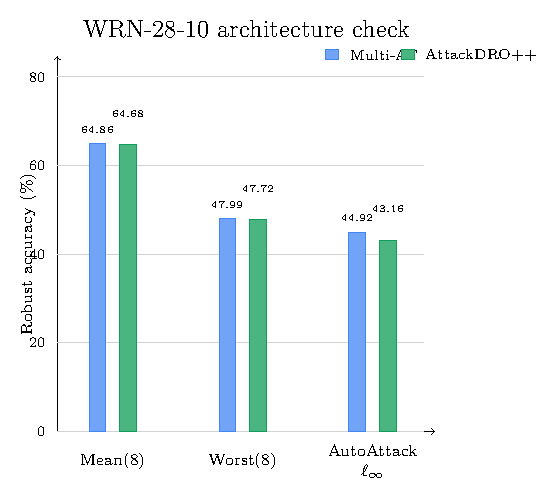
\includegraphics[width=0.75\linewidth]{figures/ablations/wrn2810_architecture_check.pdf}
    \caption[Supplementary WRN-28-10 architecture check]{Supplementary WRN-28-10 architecture check on CIFAR-10. Values are from a single run and are therefore not included in the main paired claims. Mean(8) and Worst(8) are computed over the eight non-AutoAttack attacks; AutoAttack-$\ell_\infty$ is reported separately.}
    \label{fig:app_wrn2810_architecture_check}
\end{figure}

%===========================================================
% APPENDIX D: COMPUTE RESOURCES AND ENVIRONMENT
%===========================================================

\chapter{Compute Resources and Environment Notes}
\label{app:compute}

The main experiments were executed through the Python and PyTorch pipeline
described in Chapter~\ref{chap:experimental_setup}.  Google Colab provided the
interactive GPU runtime, while Google Drive stored checkpoints, cached
adversarial examples, result CSV files, and exported figures.  The exact GPU
model available to a run was treated as execution metadata rather than an
experimental variable; model selection and statistical comparisons are based on
saved checkpoints and fixed evaluation scripts, not on wall-clock runtime.

The implementation stack used PyTorch and torchvision for training, TorchAttacks
and dedicated AutoAttack/DDN implementations for adversarial evaluation,
scikit-learn for MiniBatch K-means, and NumPy, pandas, matplotlib, and
SciencePlots for aggregation and figure generation.  Weights \& Biases was used
for telemetry and configuration tracking.  The source attack definitions,
evaluation attack suite, seed protocol, and reporting metrics are fixed in
Chapter~\ref{chap:experimental_setup}; this appendix records the compute context
only to avoid leaving the environment notes implicit.
